%% ---------------------------------------------------------------------------
%% proposal.tex
%%
%% Research Proposal, main document.
%%
%% ---------------------------------------------------------------------------
\documentclass[12pt,letterpaper]{article}
\usepackage[english]{babel}     % supports english, but default is
% \usepackage[spanish]{babel}
% include this if you want to import graphics files with /includegraphics

\usepackage{longtable}
\usepackage{ifpdf}
\usepackage[table]{xcolor}

\usepackage{anysize}
\marginsize{2.5cm}{2.5cm}{1cm}{1cm}
\usepackage{textcomp}
\usepackage{url}
\bibliographystyle{unsrt}
\usepackage{graphics}
\usepackage{amssymb}
\usepackage{graphicx}
%\usepackage{slashbox}
\usepackage[latin1]{inputenc}
\usepackage{tikz}
\usetikzlibrary{arrows,positioning}
% Color and strikethrough



\usepackage{color}
\usepackage{soul}

\usepackage{array}
\usepackage{makecell}

\usepackage{sectsty}
\allsectionsfont{\sffamily}

\definecolor{dblue}{RGB}{0,102,153}
\newcommand{\dB}[1]{\textcolor{dblue}{\textbf{#1}}}



\setlength{\parskip}{1em}

% Nombre del Estudiante
\newcommand{\scriptAuthor}{Daniel Moya S�nchez}

% T��tulo de la tesis
\newcommand{\scriptTitle}{Project Plan} 


% Keywords
\newcommand{\scriptKeywords}{key, words, ...}

% Para el PDF (cambiar si se desea otras cosas a lo indicado arriba
\newcommand{\pdfAuthor}{\scriptAuthor}
\newcommand{\pdfTitle}{\scriptTitle} 
\newcommand{\pdfKeywords}{\scriptKeywords}


\tikzset{
    mynode/.style={rectangle,rounded corners,draw=black, top color=white, bottom color=yellow!50,very thick, inner sep=1em, minimum size=3em, text centered},
    myarrow/.style={->, >=latex', shorten >=1pt, thick},
    mylabel/.style={text width=7em, text centered} 
} 

\begin{document}
 
 \graphicspath{{./}{./fig/}}

 %% ---------------------------------------------------------------------------
%% titlepage.tex
%%
%% Title page
%%
%% ---------------------------------------------------------------------------

\thispagestyle{empty} 

\begin{center}

\textsc{\LARGE Instituto Tecnol\'ogico de Costa Rica} \\
\textsc{\Large Computer Engineering Academic Area}

\textsc{\Large Proyecto de Dise\~no en Ingenier\'ia en Computadores}


\par\vspace{20mm}

\includegraphics[scale=0.25]{logoTEC}

\par\vspace*{\fill}

{\LARGE\bf{\textsf{ \Huge \scriptTitle}}}

\par\vspace*{\fill}

%Master Thesis {\sf Proposal} \\ 
%in fulfillment of the requirements for the degree of
%Plan de Proyecto
%Master of Science in Electronics Engineering \\
%Emphasis on Embedded Systems

%\par\vspace{20mm}

\textsc{\Large \scriptAuthor}

\vspace*{\fill}

{\today}

\end{center}
\newpage 
\cleardoublepage  


%  \tableofcontents

 \clearpage

% El nombre del proyecto es preciso, conciso y no ambiguo
\section{Name of the project}

Design of Application Specific Instruction Set Processors (ASIPs) for Approximate Computing


% Se identifica claramente la instituci�n donde se realizar� el proyecto
\section{Name of the institution}
\begin{itemize}
	\item Chair for Embedded System (CES), Kalrsruhe Institute of Technology (KIT), 
	Germany, and 
	\item Laboratorio Sistemas Embebidos y Electr�nica Digital (SEED-Lab) of Instituto 
	Tecnol�gico de Costa Rica (ITCR).
\end{itemize}




% Se identifica claramente qu� informaci�n se puede publicar, qu�
% informaci�n se puede compartir de manera limitada y qu�
% informaci�n se puede compartir si se firma un acuerdo de
% confidencialidad.
\section{Confidentiality requirements}

Due to the academic nature of this project, there are no special confidentiality 
requirements. However, results will not be published until the end of the project's work.




% El problema se describe de manera detallada, identificando los
% antecedentes, el contexto, usuarios, restricciones as� como otros
% aspectos relevantes para la resoluci�n del mismo.

% OPCIONAL: Se presenta una descripci�n del estado del arte de
% las investigaciones sobre el tema en cuesti�n.
\section{Problem description}

An ASIP is a processor that uses an application-specific instruction set, this means 
that, although it can execute a wide range of applications, it is optimized for a 
specific one, in which the ASIP can execute with improved performance (for instance, 
energy consumption or execution time) compared to a General Purpose Proccesor (GPP). 
Although Application Specific Integrated Circuits (ASICs) present better performance 
results, ASIPs possess flexibility. Optimizations for an ASIP can be seen in different forms, 
including \cite{henkel2003closing}: 

\begin{itemize}
 \item Instruction extension: Customized instructions can be made to extend the base Instruction Set Architecture (ISA).
 
 \item Inclusion or exclusion of predefined blocks: Not only specific software can be added 
 to extend an architecture but also customized hardware in the form of specialized blocks; 
 also, regular blocks not used can be excluded.
 
 \item Parameterization: Certain variables, such as cache sizes or number of registers, can 
 be customized to adjust for a specific application.
\end{itemize}

ASICs represent a hardware solution to a problem which is very limited and have high 
costs and a high time-to-market, but achieve the greatest performance. Contrary, GPPs 
are seen as a software solution which are very flexible but they are the least efficient. 
ASIPs are in the middle of these two as they balance flexibility and performance to have a 
good trade-off between those variables. 


The relationship between GPPs, ASIPs, and ASICs is shown in figure \ref{fig:gaa}.
Approximate computing can also be implemented on GPPs, due to their extremely flexible nature,
however, since they execute everything in software, specialized hardware modules cannot help
the performance of these systems. ASIPs can adjust to specific requirements of
a given application (through extended instructions) so that the best balance between cost savings and 
amount of error is achieved. This project focuses on that goal, to design ASIPs for a set 
of error-tolerant applications.

\begin{figure}
\begin{center}
 \includegraphics[width=\linewidth]{GPP-ASIP-ASIC}
 \caption{Comparison between GPPs, ASIPs, and ASICs \cite{henkel2006design}} \label{fig:gaa}
 \end{center}
\end{figure}

%ASIPs can also be used to adjust the balance between acceptable amount of error vs. the 
%cost (economic, area, execution time) of an application; which is is the main focus of 
%study of the project. Since different types of applications vary significantly in their 
%requirements and specifications (e.g. where the error-tolerant section is), different ASIPs 
%have to be build for each one of them so that the best balance between cost savings and 
%amount of error is achieved. This project focuses on that goal, to design ASIPs for a set 
%of error-tolerant applications.

The environment in which the ASIPs will be developed consists of several software tools 
which include Design Compiler and Prime Time from Synopsys, ModelSim from Mentor 
Graphics, ASIPMeister, CoSy compiler, Xilinx ISE and the hardware platform will be a Xilinx 
Virtex-V board. Regardless of these limitations, the project will allow for a custom hardware 
components choice with its design for specific sections. Also, for the error tolerant 
applications found, the software implementation and the tests for the general system will 
be able to be chosen between different options.

The environment in which the ASIPs will be developed consists of several software tools 
which include Design Compiler and Prime Time from Synopsys, ModelSim from Mentor 
Graphics, ASIPMeister, CoSy compiler, Xilinx ISE and the hardware platform will be a Xilinx 
Virtex-V board. Despite these restrictions, several different hardware designs can be used
for specific application sections; as well as the implementation of said applications.

Since approximated computing is still in its infancy, a lot of research and testing is still needed, 
so the users of the developed ASIPs are the same research groups of which this 
project is a part of. This project is expected to help make approximated computing a more 
solid tendency.



\section{Objectives}

% El objetivo general es directamente trazable al problema planteado, es claro, conciso.
\subsection{General objectives}
Explore the design of Application-Specific Instruction Set Processors (ASIPs) for 
error-resilient applications.


% Los objetivos espec�ficos son suficientes y consistentes con el
% objetivo general
\subsection{Specific objectives}

This project has the following specific objectives:

\begin{enumerate}
 \item Select 3 error-tolerant applications to be evaluated. 
 
 \item Develop, for each application, at least 1 instance of approximated hardware for error-tolerant sections. 
 
 \item Develop ASIP configurations using specific approximated instructions for the 
 selected applications.
 
 \item Evaluate if the gain of the execution time, area, and power consumption
 is worth the error introduced by the approximate instructions.
\end{enumerate}



% La identificaci�n de los involucrados y sus relaciones con el
% proyecto es detallada. Las relaciones se describen en detalle,
% se�alando cu�l es el inter�s del involucrado.
\section{Project stakeholders}

Due to this project belonging to a research project, there are only a few stakeholders, who 
are described below:

\begin{itemize}
 \item Jorge Castro: He is the project's supervisor and he has the general idea about the 
 project itself and guides its course. He attempts to create new knowledge with the use of 
 ASIPs for error-tolerant applications, using approximate computing techniques, and that 
 their design become automated.
 
 \item Sajjad Hussain: He works with Jorge Castro on the general guidance of the project. 
 He supports any issue with the tools in Germany so that the process of using the 
 developing platform (ASIPMeister, Dlxsim, etc.) remains smooth. He has the same interest 
 as Jorge Castro regarding the project.  
 
 \item Jeferson Gonz�lez: He is the project's supervisor at the ITCR, and the person in 
 charge of the SEED laboratory, from where he occasionally provides guidance and 
 collaboration (such as lab equipment).
 
\end{itemize}



% Se presenta una descripci�n de la soluci�n propuesta en
% correspondencia con el problema planteado y los objetivos.
% Se utilizan diagramas de bloques u otra informaci�n que permita
% visualizar la estrategia de soluci�n al problema planteado.

% OPCIONAL: Se pressentan varias alternativas de soluci�n a estudiar.
\section{Solution description}
First, an application that can have an approximated behavior in any of its steps needs to be found, for this, 
several applications have to be examined and each needs to have source code that, without 
modifications, executes correctly in standard hardware blocks. Next, the selected application 
must be studied to determine whether an entire section can be approximated, only a certain operation can be approximated (e.g. 
a matrix multiplication), or if both can be approximated. Figure \ref{fig:sol} shows a generic system  where the latter is true. 

\begin{figure}[h!]
\centering
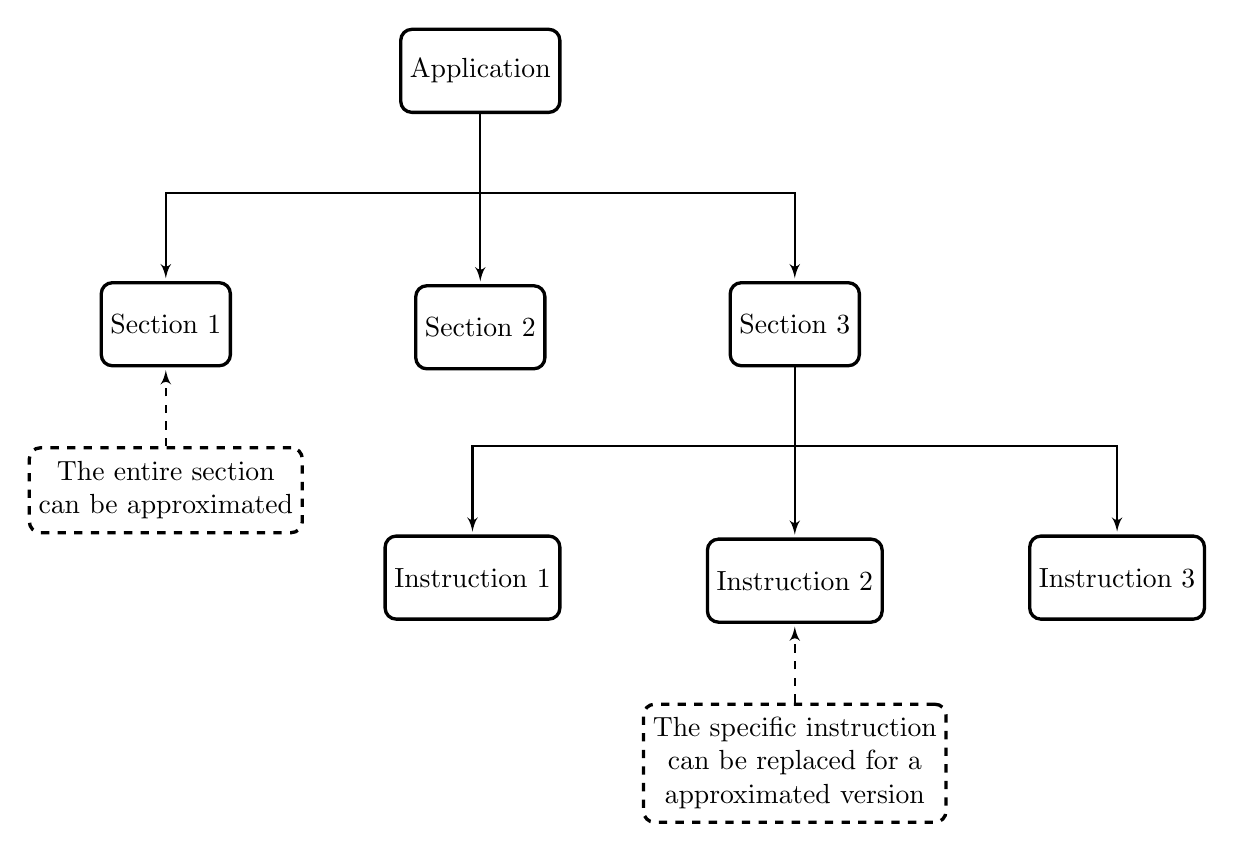
\begin{tikzpicture}[node distance=1cm, auto]  
\tikzset{
    mynode/.style={rectangle,rounded corners,draw=black, very thick, minimum size=3em, text centered},
    myarrow/.style={->, >=latex', shorten >=1pt, thick},
    mylabel/.style={text width=7em, text centered} 
}  
\node[mynode] (manufacturer) {Application};  
\node[mynode, below left =3cm of manufacturer] (section1) {Section 1}; 
\node[mynode, below=2.16cm of manufacturer] (section2) {Section 2};
\node[mynode, below right=3cm of manufacturer] (section3) {Section 3};

\node[mynode, below=1cm of section1, dashed] (comment1) {\makecell{The entire section \\ can be approximated}};

\node[mynode, below left=3cm of section3] (instru1) {Instruction 1};
\node[mynode, below =2.16cm of section3] (instru2) {Instruction 2};
\node[mynode, below right=3cm of section3] (instru3) {Instruction 3};

\node[mynode, below=1cm of instru2, dashed] (comment2) {\makecell{The specific instruction \\ can be replaced for a \\ approximated version}};


\draw[myarrow] (manufacturer.south)  -- ++(0,-1) -|  (section1.north);
\draw[myarrow] (manufacturer.south)   -|  (section2.north);
\draw[myarrow] (manufacturer.south)  -- ++(0,-1) -|  (section3.north); 

\draw[->, >=latex', shorten >=1pt, thick, dashed]  (comment1.north) -|  (section1.south); 

\draw[myarrow] (section3.south)  -- ++(0,-1) -|  (instru1.north);
\draw[myarrow] (section3.south)   -|  (instru2.north);
\draw[myarrow] (section3.south)  -- ++(0,-1) -|  (instru3.north); 
 
 \draw[->, >=latex', shorten >=1pt, thick, dashed]  (comment2.north) -|  (instru2.south); 
 
\end{tikzpicture} 
\medskip
\caption{A possible situation to solve with this project} 
\label{fig:sol}
\end{figure}


As seen in figure \ref{fig:sol}, that example of an application has three sections, from which the first one (this could be a preprocessing stage)
can be entirely approximated, the second one cannot be approximated at all (we can think of this as a critical section of the application)
and finally, in the third second, three specific instructions can be seen, from which the second one has a approximated version. The specific
characteristics of the final applications selected have to be determined to execute an analysis similar to this one presented. 

Once the approximate parts have been selected, the process of creating the ASIPs begin. These ASIPs are continuously tested to ensure
that the application does not exceed a certain error threshold, but also, that a greater performance in energy, area or execution time is achieved compared to the
original version. 

Other solutions have been proposed, which include randomness in programs and inference via probabilistic programming as software solutions;
approximate computing with GPPs (as discussed in the problem description section) as a different processor architecture solution;
improvements in the memory, storage, and interconnections for simplier circuits and finally neural accelerators as a different approximate
computing paradigm \cite{xu2018approximate}.


% Los entregables con consistentes con los objetivos del proyecto y
% con los productos de un proyecto de ingenier�a de software para
% efectos de desarrollo posterior o mantenimiento.
% Los entregables tienen un identificador �nico.
% Los entregables deben incluir:
%	- Documento de Requerimientos
%	- Documento de Dise�o
%	- Plan de pruebas/Resultados de las preubas
%	- Otra documentaci�n relevante: instrucciones de compilaci�n,
% manuales de instalaci�n, manual de usuario etc.
\section{Deliverables and criteria of acceptance}

The expected deliverables are presented in table \ref{tab:del}.

\begin{table}[h!]
\begin{center}
\caption{Deliverables with the corresponding criteria of acceptance}
\begin{tabular}{|c|c|c|} 
 \hline
 Name & Description & Criteria of acceptance \\ \hline
 Deliverable-01 & List of selected approximate applications & \makecell{Approval given by the \\ supervisor} \\ \hline
 Deliverable-02 & Instances of approximated hardware & \makecell{Approval given by the \\ supervisor} \\ \hline
 Deliverable-03 & Configuration of approximated ASIPs & \makecell{Approval given by the \\ supervisor} \\ \hline 
 Deliverable-04 & \makecell{Comparison and analysis of \\
 obtained results (execution time,\\ area and power vs error)} & \makecell{Execution of the test plan \\ with satisfying results}  \\ \hline %Plan Prueba
 Deliverable-05 & Project Plan document & \makecell{Specifications given by the \\ professors for this document} \\ \hline
 Deliverable-06 & Requirements document & \makecell{Specifications given by the \\ professors for this document} \\ \hline
 Deliverable-07 & Design document & \makecell{Specifications given by the \\ professors for this document} \\ \hline
 Deliverable-08 & Test plan document & \makecell{Specifications given by the \\ supervisor for this document} \\ \hline
 Deliverable-09 & Final report & \makecell{Specifications given by the \\ professor for this document} \\ \hline
\end{tabular}
\label{tab:del}
\end{center}
\end{table}



% Las cuatro �reas analizadas (personal, herramientas, procesos,
% insumos) son analizadas en detalle, identificando los riesgos m�s
% sobresalientes para cada una de esas �reas. Para cada riesgo se
% indica la probabilidad y el impacto para el proyecto.
\section{Risk analysis}

Since most of the work is done from home (\emph{ssh} to the Germany server) or at the SEED laboratory, few risks are considered. Table \ref{tab:risk} summarizes
this information.

\begin{table}[h!]
\begin{center}
\caption{Risk analysis}
\begin{tabular}{ | c | c | c | c | c | } 
 \hline
 Risk & Type & \makecell{Probability of \\ occurrence} & \makecell{Impact \\ (hours)} & \makecell{Risk exposure \\ (hours)} \\
 \hline
 \makecell{Illness or any special \\ medical condition} & Personal & 0.5 & 8 & 4 \\ \hline
 \makecell{Difficulties understanding \\ ASIP-related concepts} & Personal & 0.5 & 8 & 4 \\ \hline
 \makecell{General server errors \\ (missing files, permission \\ restrictions, etc)} & Tools & 0.75 & 24 & 18 \\ \hline
 \makecell{Delays when acquiring \\ the hardware platform} &Tools & 0.25 & 8 & 2 \\ \hline
 \makecell{ASIP configurations that \\ exceed error threshold} & Methods & 0.75 & 8 & 6 \\ \hline
 \makecell{Delays when acquiring the \\ server environment set} & Inputs & 0.75 & 8 & 6 \\ \hline
\end{tabular}
\label{tab:risk}
\end{center}
\end{table}



% Las actividades propuestas son consistentes con los objetivos
% espec�ficos.
% Las estimaciones de esfuerzos son proporcionales con la
% complejidad o el tama�o de las mismas.
% Se asigna un identificador �nico (c�digo) a cada actividad.
\section{Activities and effort budget}

This section takes in consideration a total of 216 engineering hours; this is calculated
by multiplying the 16 weeks by 12 extra-class hours, and then adding 4 hours times
6 because of the 6 weeks that there is no class attendance. These hours are then distributed
among all the tasks, considering a risk reserve. Table \ref{tab:act} summarizes all the 
activities for the project.

\begin{table}[h!]
\begin{center}
\caption{Activities and effort budget}
\begin{tabular}{ | c | c | c | c | c | } 
 \hline
 ID  &Activity & \makecell{Engineering \\ hours} & \makecell{Risk reserve \\ (hours)} & \makecell{Total \\ (hours)} \\ \hline
 01 & \makecell{Get to know the software platform} & 30 & 2 & 32 \\ \hline
 02 & \makecell{Find appropiate error-tolerant applications \\ and identify the sections that can be \\ 
  approximated} & 30 & 2 & 32  \\ \hline
 03 & \makecell{Implement the ASIPs in the error \\ tolerant applications found} & 60 & 4 & 64 \\ \hline
 03 & \makecell{Compare execution time, area and power \\ vs error in selected applications} & 38 & 2 & 40 \\ \hline
 04 & \makecell{Redact Project Plan document} & 8 & 0 & 8 \\ \hline
 05 & \makecell{Redact Requirements document} & 8 & 0 & 8 \\ \hline
 06 & \makecell{Redact Design document} & 8 & 0 & 8 \\ \hline
 07 & \makecell{Redact Test plan document} & 8 & 0 & 8 \\ \hline
 08 & \makecell{Redact Final documentation} & 15 & 1 & 16 \\ \hline \hline
 \multicolumn{4}{|c|}{Result} & 216 \\ \hline
\end{tabular}
\label{tab:act}
\end{center}
\end{table}



% El cronograma incluye todas las actividades y las mismas no
% guardan una consistecia l�gica para la construcci�n de los
% entregables.
% Se incluyen hitos para los entregables m�s sobresalientes.
% El nivel de granularidad de las actividades ofrece suficiente detalle.
% Al menos una actividad por semana.
\section{Schedule}

Considering the 4 months (16 weeks) of the semester, the project is scheduled as shown in figure \ref{tab:schd}, where
the light blue color represents the initial tasks for the project, blue the development of the project itself and
gray documentation tasks. 

\begin{table}[h!]
\begin{center}
\caption{Schedule for the entire project}
\begin{tabular}{ | c | c | c | c | c | c | c | c | c | c | c | c | c | c | c | c | c |} 
 \hline
   & \multicolumn{16}{|c|}{Week} \\
 \hline
 Activity & 1 & 2 & 3 & 4 & 5 & 6 & 7 & 8 & 9 & 10 & 11 & 12 & 13 & 14 & 15 & 16 \\ \hline
 \makecell{Reading the corresponding \\ literature about the \\ project and understanding \\ the concept of ASIPs}
 & \cellcolor[HTML]{5B9BD5}  & \cellcolor[HTML]{5B9BD5} &  &  &  &  &  &  &  &  &  &  &  &  &  &  \\ \hline
 \makecell{Execution of the laboratory \\ script to get  to know \\ the software tools like \\ ASIPMeister, Dlxsim, etc}
 & \cellcolor[HTML]{5B9BD5}  & \cellcolor[HTML]{5B9BD5}  & \cellcolor[HTML]{5B9BD5} &  &  &  &  &  &  &  &  &  &  &  &  &  \\ \hline
 \makecell{Delivery of the ``Plan Project'' \\ document}
 &  & \cellcolor[HTML]{A5A5A5}  &  &  &  &  &  &  &  &  &  &  &  &  &  &  \\ \hline
 \makecell{Delivery of the ``Requirements'' \\ document}
 &  &   & \cellcolor[HTML]{A5A5A5} &  &  &  &  &  &  &  &  &  &  &  &  &  \\ \hline
 \makecell{Delivery of the ``Design'' \\ document}
 &  &   &  & \cellcolor[HTML]{A5A5A5} &  &  &  &  &  &  &  &  &  &  &  &  \\ \hline
  \makecell{Research of error-tolerant \\ applications with desirable \\ features}
 &  &   &  & \cellcolor[HTML]{4472C4} & \cellcolor[HTML]{4472C4} & \cellcolor[HTML]{4472C4} &  &  &  &  &  &  &  &  &  &  \\ \hline
   \makecell{Design of blocks with  \\ special approximated \\ instructions}
 &  &   &  &  &  &  & \cellcolor[HTML]{4472C4} & \cellcolor[HTML]{4472C4} & \cellcolor[HTML]{4472C4} &  &  &  &  &  &  &  \\ \hline
    \makecell{Putting the blocks together  \\ to build the ASIPs}
 &  &   &  &  &  &  &  &  &  & \cellcolor[HTML]{4472C4} & \cellcolor[HTML]{4472C4} & \cellcolor[HTML]{4472C4} &  &  &  &  \\ \hline
     \makecell{Final results comparison} &  &   &  &  &  &  &  &  &  &  &  &
     \cellcolor[HTML]{4472C4} & \cellcolor[HTML]{4472C4} & \cellcolor[HTML]{4472C4} & \cellcolor[HTML]{4472C4} &  \\ \hline
  \makecell{Delivery of the ``Final report'' \\ document}
 &  &   &  &  &  &  &  &  &  &  &  &  &  &  & \cellcolor[HTML]{A5A5A5} & \cellcolor[HTML]{A5A5A5} \\ \hline
 \end{tabular}
\label{tab:schd}
\end{center}
\end{table}


% Referencias del Background y el Related Work
\bibliographystyle{sty/plainurl}
\bibliography{references}



\end{document}

